\documentclass{article}
\usepackage{graphics} 
\usepackage{hyperref}

\author{Kevin Zollicoffer}
\title{Predictive Modeling\\Lesson 3\\\emph{Logistical Regression and Neural Networks}}
\date{09/29/2013}

\usepackage{Sweave}
\begin{document}
\maketitle
%\tableofcontents
\Sconcordance{concordance:LogisticalRegression.tex:LogisticalRegression.Rnw:%
1 8 1 1 0 15 1 1 2 1 0 1 1 40 0 1 2 2 1 1 2 1 0 5 1 3 0 1 2 2 1 1 2 1 0 %
3 1 3 0 1 2 3 1 1 2 1 0 1 2 39 0 1 2 73 0 1 2 49 0 1 2 208 0 1 3 2 1 1 %
2 1 0 1 1 7 0 1 2 2 1 1 2 1 0 2 1 36 0 1 2 1 1 1 2 1 0 3 1 3 0 1 2 3 1 %
1 2 1 0 1 1 3 0 1 2 2 1 1 9 7 0 1 6 4 0 2 1 401 0 1 2 17 1}


\section*{Introduction}
The RStudio project files and accompanying artifacts, including the tex file that created this PDF, are publicly available on GitHub
\\
\url{https://github.com/zollie/PASS-PredictiveModeling-LogisticalRegression}

\section*{Data Setup}
I took the Excel spreadsheet and saved it as a CSV for easy import into R
\begin{Schunk}
\begin{Sinput}
> gc <- read.csv("~/R/PASS/PredictiveModeling/LogisticRegression/GermanCredit.csv")
> head(gc)
\end{Sinput}
\begin{Soutput}
  OBS. CHK_ACCT DURATION HISTORY NEW_CAR USED_CAR FURNITURE RADIO.TV EDUCATION
1    1        0        6       4       0        0         0        1         0
2    2        1       48       2       0        0         0        1         0
3    3        3       12       4       0        0         0        0         1
4    4        0       42       2       0        0         1        0         0
5    5        0       24       3       1        0         0        0         0
6    6        3       36       2       0        0         0        0         1
  RETRAINING AMOUNT SAV_ACCT EMPLOYMENT INSTALL_RATE MALE_DIV MALE_SINGLE
1          0   1169        4          4            4        0           1
2          0   5951        0          2            2        0           0
3          0   2096        0          3            2        0           1
4          0   7882        0          3            2        0           1
5          0   4870        0          2            3        0           1
6          0   9055        4          2            2        0           1
  MALE_MAR_or_WID CO.APPLICANT GUARANTOR PRESENT_RESIDENT REAL_ESTATE
1               0            0         0                4           1
2               0            0         0                2           1
3               0            0         0                3           1
4               0            0         1                4           0
5               0            0         0                4           0
6               0            0         0                4           0
  PROP_UNKN_NONE AGE OTHER_INSTALL RENT OWN_RES NUM_CREDITS JOB NUM_DEPENDENTS
1              0  67             0    0       1           2   2              1
2              0  22             0    0       1           1   2              1
3              0  49             0    0       1           1   1              2
4              0  45             0    0       0           1   2              2
5              1  53             0    0       0           2   2              2
6              1  35             0    0       0           1   1              2
  TELEPHONE FOREIGN RESPONSE
1         1       0        1
2         0       0        0
3         0       0        1
4         0       0        1
5         0       0        0
6         1       0        1
\end{Soutput}
\end{Schunk}

\noindent
The categorical predictors are turned into factors for R
\begin{Schunk}
\begin{Sinput}
> gc$RESPONSE <- factor(gc$RESPONSE)
> gc$JOB <- factor(gc$JOB)
> gc$EMPLOYMENT <- factor(gc$EMPLOYMENT)
> gc$SAV_ACCT <- factor(gc$SAV_ACCT)
> gc$HISTORY <- factor(gc$HISTORY)
> gc$CHK_ACCT <- factor(gc$CHK_ACCT)
\end{Sinput}
\end{Schunk}

\section*{Partitioning}
Next, the data is paritioned into 60\% Train and 40\% Test sets. I set the RNG seed for reproducibility
\begin{Schunk}
\begin{Sinput}
> n <- nrow(gc)
> a <- sort(sample(1:n, floor(n*.6)))
> gc.train <- gc[a,]
> gc.test <- gc[-a,]
\end{Sinput}
\end{Schunk}

\section*{Logistical Regression}
A Logistical Regression model is fit to the train data. 

\begin{Schunk}
\begin{Sinput}
> logit <- glm(RESPONSE ~ CHK_ACCT+DURATION+HISTORY+NEW_CAR+USED_CAR+FURNITURE+RADIO.TV+EDUCATION+RETRAINING+AMOUNT+SAV_ACCT+EMPLOYMENT+INSTALL_RATE+MALE_DIV+MALE_SINGLE+MALE_MAR_or_WID+CO.APPLICANT+GUARANTOR+PRESENT_RESIDENT+REAL_ESTATE+PROP_UNKN_NONE+AGE+OTHER_INSTALL+RENT+OWN_RES+NUM_CREDITS+JOB+NUM_DEPENDENTS+TELEPHONE+FOREIGN, data=gc.train, family=binomial("logit"))
> logit
\end{Sinput}
\begin{Soutput}
Call:  glm(formula = RESPONSE ~ CHK_ACCT + DURATION + HISTORY + NEW_CAR + 
    USED_CAR + FURNITURE + RADIO.TV + EDUCATION + RETRAINING + 
    AMOUNT + SAV_ACCT + EMPLOYMENT + INSTALL_RATE + MALE_DIV + 
    MALE_SINGLE + MALE_MAR_or_WID + CO.APPLICANT + GUARANTOR + 
    PRESENT_RESIDENT + REAL_ESTATE + PROP_UNKN_NONE + AGE + OTHER_INSTALL + 
    RENT + OWN_RES + NUM_CREDITS + JOB + NUM_DEPENDENTS + TELEPHONE + 
    FOREIGN, family = binomial("logit"), data = gc.train)

Coefficients:
     (Intercept)         CHK_ACCT1         CHK_ACCT2         CHK_ACCT3  
       0.0130190         0.6274385         1.5478081         1.7756171  
        DURATION          HISTORY1          HISTORY2          HISTORY3  
      -0.0213973         0.6218902         1.0542574         0.9128612  
        HISTORY4           NEW_CAR          USED_CAR         FURNITURE  
       1.9196216        -0.2966938         1.5245519         0.7469575  
        RADIO.TV         EDUCATION        RETRAINING            AMOUNT  
       0.6227738        -0.3288723         0.3219821        -0.0001606  
       SAV_ACCT1         SAV_ACCT2         SAV_ACCT3         SAV_ACCT4  
       0.1330299         0.3061612         1.2335501         1.0533710  
     EMPLOYMENT1       EMPLOYMENT2       EMPLOYMENT3       EMPLOYMENT4  
      -0.2979299         0.1749510         0.4841481        -0.2144694  
    INSTALL_RATE          MALE_DIV       MALE_SINGLE   MALE_MAR_or_WID  
      -0.3948298         0.1672193         0.7121614         0.1611906  
    CO.APPLICANT         GUARANTOR  PRESENT_RESIDENT       REAL_ESTATE  
      -0.7918356         0.9532831         0.0169459         0.5110658  
  PROP_UNKN_NONE               AGE     OTHER_INSTALL              RENT  
      -0.1388947         0.0097773        -0.4422190        -0.2464168  
         OWN_RES       NUM_CREDITS              JOB1              JOB2  
       0.2746791         0.0027873        -0.2988528        -0.2699509  
            JOB3    NUM_DEPENDENTS         TELEPHONE           FOREIGN  
       0.2313653        -0.4014251         0.4155514         0.3403382  

Degrees of Freedom: 599 Total (i.e. Null);  556 Residual
Null Deviance:	    724.4 
Residual Deviance: 520.1 	AIC: 608.1
\end{Soutput}
\begin{Sinput}
> summary(logit)
\end{Sinput}
\begin{Soutput}
Call:
glm(formula = RESPONSE ~ CHK_ACCT + DURATION + HISTORY + NEW_CAR + 
    USED_CAR + FURNITURE + RADIO.TV + EDUCATION + RETRAINING + 
    AMOUNT + SAV_ACCT + EMPLOYMENT + INSTALL_RATE + MALE_DIV + 
    MALE_SINGLE + MALE_MAR_or_WID + CO.APPLICANT + GUARANTOR + 
    PRESENT_RESIDENT + REAL_ESTATE + PROP_UNKN_NONE + AGE + OTHER_INSTALL + 
    RENT + OWN_RES + NUM_CREDITS + JOB + NUM_DEPENDENTS + TELEPHONE + 
    FOREIGN, family = binomial("logit"), data = gc.train)

Deviance Residuals: 
    Min       1Q   Median       3Q      Max  
-2.9686  -0.6543   0.3575   0.6694   2.1016  

Coefficients:
                   Estimate Std. Error z value Pr(>|z|)    
(Intercept)       1.302e-02  1.605e+00   0.008 0.993529    
CHK_ACCT1         6.274e-01  2.846e-01   2.205 0.027471 *  
CHK_ACCT2         1.548e+00  5.064e-01   3.057 0.002239 ** 
CHK_ACCT3         1.776e+00  3.051e-01   5.821 5.86e-09 ***
DURATION         -2.140e-02  1.302e-02  -1.644 0.100179    
HISTORY1          6.219e-01  7.124e-01   0.873 0.382692    
HISTORY2          1.054e+00  5.711e-01   1.846 0.064890 .  
HISTORY3          9.129e-01  6.232e-01   1.465 0.142966    
HISTORY4          1.920e+00  5.942e-01   3.231 0.001235 ** 
NEW_CAR          -2.967e-01  6.039e-01  -0.491 0.623239    
USED_CAR          1.525e+00  7.304e-01   2.087 0.036868 *  
FURNITURE         7.470e-01  6.284e-01   1.189 0.234582    
RADIO.TV          6.228e-01  6.049e-01   1.029 0.303258    
EDUCATION        -3.289e-01  7.172e-01  -0.459 0.646553    
RETRAINING        3.220e-01  6.680e-01   0.482 0.629820    
AMOUNT           -1.606e-04  6.272e-05  -2.560 0.010471 *  
SAV_ACCT1         1.330e-01  3.926e-01   0.339 0.734702    
SAV_ACCT2         3.062e-01  5.367e-01   0.570 0.568363    
SAV_ACCT3         1.234e+00  6.603e-01   1.868 0.061757 .  
SAV_ACCT4         1.053e+00  3.452e-01   3.051 0.002278 ** 
EMPLOYMENT1      -2.979e-01  6.147e-01  -0.485 0.627913    
EMPLOYMENT2       1.750e-01  6.060e-01   0.289 0.772825    
EMPLOYMENT3       4.841e-01  6.461e-01   0.749 0.453681    
EMPLOYMENT4      -2.145e-01  5.992e-01  -0.358 0.720383    
INSTALL_RATE     -3.948e-01  1.165e-01  -3.390 0.000699 ***
MALE_DIV          1.672e-01  5.252e-01   0.318 0.750180    
MALE_SINGLE       7.122e-01  2.872e-01   2.480 0.013136 *  
MALE_MAR_or_WID   1.612e-01  4.036e-01   0.399 0.689600    
CO.APPLICANT     -7.918e-01  4.855e-01  -1.631 0.102869    
GUARANTOR         9.533e-01  5.439e-01   1.753 0.079671 .  
PRESENT_RESIDENT  1.695e-02  1.175e-01   0.144 0.885307    
REAL_ESTATE       5.111e-01  2.919e-01   1.751 0.079948 .  
PROP_UNKN_NONE   -1.389e-01  5.371e-01  -0.259 0.795927    
AGE               9.777e-03  1.242e-02   0.788 0.430972    
OTHER_INSTALL    -4.422e-01  2.787e-01  -1.587 0.112531    
RENT             -2.464e-01  6.414e-01  -0.384 0.700847    
OWN_RES           2.747e-01  6.029e-01   0.456 0.648703    
NUM_CREDITS       2.787e-03  2.402e-01   0.012 0.990743    
JOB1             -2.989e-01  9.660e-01  -0.309 0.757048    
JOB2             -2.700e-01  9.374e-01  -0.288 0.773358    
JOB3              2.314e-01  9.346e-01   0.248 0.804472    
NUM_DEPENDENTS   -4.014e-01  3.255e-01  -1.233 0.217500    
TELEPHONE         4.156e-01  2.630e-01   1.580 0.114081    
FOREIGN           3.403e-01  7.422e-01   0.459 0.646558    
---
Signif. codes:  0 ‘***’ 0.001 ‘**’ 0.01 ‘*’ 0.05 ‘.’ 0.1 ‘ ’ 1

(Dispersion parameter for binomial family taken to be 1)

    Null deviance: 724.36  on 599  degrees of freedom
Residual deviance: 520.15  on 556  degrees of freedom
AIC: 608.15

Number of Fisher Scoring iterations: 5
\end{Soutput}
\begin{Sinput}
> confint(logit)
\end{Sinput}
\begin{Soutput}
                         2.5 %        97.5 %
(Intercept)      -3.1088217929  3.205295e+00
CHK_ACCT1         0.0730383976  1.190740e+00
CHK_ACCT2         0.6033382534  2.608454e+00
CHK_ACCT3         1.1893883645  2.388138e+00
DURATION         -0.0471800654  4.028345e-03
HISTORY1         -0.7641375436  2.043542e+00
HISTORY2         -0.0420924161  2.213788e+00
HISTORY3         -0.2860916509  2.170036e+00
HISTORY4          0.7802222009  3.123767e+00
NEW_CAR          -1.5256645097  8.645935e-01
USED_CAR          0.0854573119  2.968877e+00
FURNITURE        -0.5220082124  1.963286e+00
RADIO.TV         -0.6057609977  1.789263e+00
EDUCATION        -1.7666887512  1.062207e+00
RETRAINING       -1.0136186649  1.624869e+00
AMOUNT           -0.0002847035 -3.794786e-05
SAV_ACCT1        -0.6231690751  9.217988e-01
SAV_ACCT2        -0.6920073338  1.440611e+00
SAV_ACCT3         0.0378169851  2.675750e+00
SAV_ACCT4         0.3951067980  1.753439e+00
EMPLOYMENT1      -1.5252554394  8.991256e-01
EMPLOYMENT2      -1.0343351917  1.356605e+00
EMPLOYMENT3      -0.7968523911  1.750967e+00
EMPLOYMENT4      -1.4174238024  9.456194e-01
INSTALL_RATE     -0.6271862178 -1.696799e-01
MALE_DIV         -0.8480863667  1.225398e+00
MALE_SINGLE       0.1522385488  1.280286e+00
MALE_MAR_or_WID  -0.6208394998  9.674190e-01
CO.APPLICANT     -1.7543180324  1.630764e-01
GUARANTOR        -0.0535686993  2.105975e+00
PRESENT_RESIDENT -0.2136948389  2.477828e-01
REAL_ESTATE      -0.0547834291  1.092135e+00
PROP_UNKN_NONE   -1.1850501887  9.279768e-01
AGE              -0.0142842077  3.450442e-02
OTHER_INSTALL    -0.9872548856  1.079713e-01
RENT             -1.5077823881  1.013876e+00
OWN_RES          -0.9061387196  1.465613e+00
NUM_CREDITS      -0.4682461593  4.782817e-01
JOB1             -2.3045383941  1.533273e+00
JOB2             -2.2278672639  1.499925e+00
JOB3             -1.7166728082  2.005040e+00
NUM_DEPENDENTS   -1.0371197579  2.424741e-01
TELEPHONE        -0.0965757578  9.364935e-01
FOREIGN          -1.0238410353  1.938145e+00
\end{Soutput}
\begin{Sinput}
> residuals(logit)
\end{Sinput}
\begin{Soutput}
          1           2           4           6           9          10 
 0.24762860 -1.21427984  0.99415371  0.78194692  0.14388602 -1.08584589 
         12          13          14          16          17          18 
-0.41187164  0.54221809 -1.21270868 -1.02217785  0.23278129  1.82708699 
         20          23          24          26          27          28 
 0.50908094  0.75460042  0.31096173  0.41574845  0.93225559  0.34908713 
         29          30          31          32          35          37 
 0.32423566 -0.70947614  0.57133002  1.08781747  0.66048002  0.66894075 
         38          39          40          42          43          44 
-1.66666261  0.35734468  0.56299870  0.59781397  0.83662433  0.60768594 
         45          46          47          48          49          50 
-0.79459969  0.60772598  0.60482268  0.46128567  0.39021223  0.71370251 
         51          53          55          58          59          60 
 0.87859713  0.37976129 -0.73886534  0.82124259  0.94087228 -0.47350270 
         61          64          65          66          67          68 
 0.62933676 -0.50793516  0.82330960  0.61503667  0.70856848  0.68839058 
         69          70          72          75          76          79 
-1.33132911  0.53336746  0.19110584 -1.38032193  0.44059609  0.66861140 
         80          81          85          86          87          90 
 1.13684281 -2.40308121  0.76400942  0.15239383  0.88821966 -1.02879570 
         91          92          93          94          95          96 
 0.22924883  0.38063697 -2.19421182  0.62746997  0.45626522 -0.24070372 
         97          98          99         100         103         105 
 0.31261933  0.91371105  0.63681670  0.46660626  0.41229081  0.22457524 
        106         113         115         117         118         124 
-1.17392065  1.21530388  0.89494465 -1.38006600  0.62009275  0.49042993 
        125         127         130         134         135         136 
-1.54602580  0.93889623 -0.95574227  0.64209963  0.73000774  0.18351204 
        137         138         139         140         142         146 
 0.24355414 -2.20380844  0.14719867  0.50381967  1.35381410  1.32126102 
        147         149         150         151         153         154 
 0.75978213  0.60113285  0.19335876  0.45733607  0.90018618  0.53986815 
        159         161         162         163         164         166 
 0.83838591  0.26214578  0.82640198  0.36600298  1.03184946  0.17685672 
        168         169         171         172         174         175 
 0.59573324  0.51680993 -0.34713454  0.37670167  0.31258457 -0.82745183 
        177         178         179         183         184         186 
 0.88698489  0.55766824  0.40669257 -1.00862405  0.11787603  0.30490007 
        187         188         190         192         193         194 
-1.54110660  0.41813025  1.07973227 -0.56101852 -1.23060219  0.34898800 
        196         197         198         199         202         206 
-1.93385685  0.18348132 -0.88726734  0.54804285  1.40193167  0.94466340 
        207         208         209         211         212         213 
 0.20698744  0.60569371  1.73684946  0.10151912  0.29105270 -0.78096448 
        215         217         218         219         220         222 
 0.23798728  1.45719464  0.35578645  1.09216514  0.45547222  1.49035945 
        223         227         228         229         232         234 
 0.41512509 -1.40237701 -1.13874246 -2.27426574  0.58053610  0.53543527 
        235         237         238         239         242         247 
 0.14686943 -1.55461797 -0.75035435  0.40734304  0.33860355  0.23490793 
        250         251         254         255         257         259 
-1.58167508  0.32897359  0.39706064  0.22581971  0.28806558  0.28420911 
        260         261         262         265         266         268 
 0.28504319  0.55213452  1.46876896  0.35655209 -1.35280874  0.85057032 
        269         271         272         273         276         277 
-1.15980608  0.35821882  0.24281990  2.10154673  0.25688979  0.33664300 
        279         280         281         282         283         285 
-2.06892280  0.40864956  0.14320935  0.30748791  0.38954531  1.19125853 
        286         287         289         291         292         294 
 1.97048387  1.21042453  0.39404435  0.25087576 -1.50869965  0.48925919 
        295         296         297         298         299         302 
 0.80685775 -0.94769654  0.30140368  0.58011798  0.24101173 -0.76700125 
        305         307         308         310         312         315 
-1.34087339  0.37540515 -1.16083247  1.27739107  0.77216528  0.25494271 
        317         320         322         324         326         330 
 0.48233411  1.14809405 -0.83483623  0.64707753  0.37833175  0.98064542 
        331         334         337         340         341         343 
 0.35767461 -1.52239299  0.65285107  0.91265019  1.34190587  0.76389926 
        344         345         346         347         349         350 
 0.73809917  0.50443526  0.41615382  0.31727211  0.22123995 -1.69532129 
        352         353         354         355         356         359 
-2.12151980  0.06599396 -0.63539061  0.62512847 -0.94457055  0.44429318 
        360         361         362         363         366         368 
-1.00484242  0.79165904  0.21919169  0.82154575  0.24290014  1.38768214 
        369         371         372         375         376         378 
-0.81147686  0.46289861  0.36079797 -0.26435426 -0.74438017  0.30907600 
        383         384         385         388         389         392 
 0.71775013  0.76757079  0.55462777  0.66005878  0.48365189  0.41902753 
        393         394         396         397         399         400 
 1.35127025  0.46300971  1.72566368  1.06983155 -1.42630069  0.19708431 
        403         404         409         411         412         413 
-1.45214533  0.73780869  0.43336537  1.18621358  0.16616668 -2.49475279 
        415         417         418         420         421         423 
-1.03945472 -0.77837582  1.41930666 -1.37669719  0.51024354  0.40503235 
        424         426         427         428         429         433 
 0.24414512  0.48387125  0.47252142  0.12040749  0.28845132  0.52352184 
        435         436         437         438         440         442 
 0.67089767 -2.55174224  0.37305800  0.29741909 -1.58959481  1.24561423 
        444         448         449         454         455         456 
-1.29067059  0.26939858  0.17507147  0.27226539 -0.96367408  0.45172766 
        458         459         461         467         470         471 
-1.67592838  1.43839020  0.63223019 -0.68829900  0.26111935 -1.12223469 
        472         475         476         477         478         479 
-0.65199980 -1.76328599 -0.66069646  0.37076908  0.80649025  0.44224778 
        480         483         484         485         486         487 
 0.73827145  1.11071114  0.25091516  0.23074367 -1.67349412  0.25496228 
        488         490         491         492         493         497 
 1.56387835  0.43845092  0.27857178 -0.67462236  0.20962751 -0.65222734 
        499         500         501         502         503         505 
 0.64070388  0.47984595 -0.45095929  1.21281975  0.33952068 -0.41146712 
        506         512         513         514         515         517 
-2.60003358  0.25644739  0.41398411  1.32806884  0.57665701  0.66405961 
        519         523         525         526         527         530 
 1.02436547 -0.43140114  0.69077622  0.80470256  0.63436379  1.03818167 
        531         534         535         537         538         539 
 1.27229983  0.44399031  0.45215652  0.72477944  0.66570123 -0.33461756 
        540         541         542         544         545         546 
 0.66799949 -1.67506690  0.88012075 -2.33191031  0.37365273 -0.76886895 
        547         549         550         553         554         555 
 0.60089871 -0.95235048  0.17138690 -1.90110866  0.95781259  0.74686988 
        557         558         559         561         563         565 
-0.54724250 -1.62349998 -1.09599189  0.83113570  0.71449080  0.65050298 
        567         568         569         570         571         573 
-1.24786076  0.16275426  0.67514066 -0.76698791 -0.85417044  0.23575863 
        574         576         578         579         581         583 
 1.44290497  0.49413023  0.31459517 -0.88726946 -2.06122386  0.59160600 
        585         586         589         590         592         594 
 0.52993720 -1.30672685 -1.28862909 -1.89843689  1.15273826 -0.85200831 
        595         597         598         600         601         602 
-1.35030344 -0.58216627 -1.70594254  0.52277949  0.37339065 -1.44661218 
        603         604         606         607         608         612 
-0.54079114 -1.93628430  1.01230862  0.16548569 -0.72702051 -1.49813426 
        614         615         616         617         618         620 
 0.77061541 -2.07401659  1.30253511  0.94891761  0.78394476  0.62023322 
        621         625         626         627         629         630 
 0.46353939 -1.21750663  0.34681135  0.19445205  0.24674001  0.22718818 
        632         633         635         636         637         640 
-1.05297614  0.63443719 -0.96964723  0.91177674  0.54321220 -0.94642238 
        641         642         643         646         649         650 
-0.90596601  1.13466379 -2.16150944 -1.48324228 -1.19488506 -0.72346344 
        651         653         654         655         657         658 
 1.73625177 -0.66034984 -1.19392405  0.15801378 -0.83277017  0.64636745 
        662         663         665         666         667         668 
-1.19630397  0.42851514  0.42191704  0.87437836  0.82892642  0.83941054 
        669         670         672         673         674         675 
-0.83108913  0.49710284  0.42202140  1.04998991  0.30105762 -1.61177524 
        678         679         681         683         684         691 
-0.94781960  1.38214472  0.63625679  0.61369541  0.55290035  0.59037445 
        693         694         695         698         700         701 
 0.79046973  0.50532072  0.39120627  0.32845743  0.77853339 -1.82780462 
        703         705         706         708         709         710 
 0.81073544  1.57289839  0.90920454 -0.54288547  0.94800833  0.51223809 
        712         714         715         716         717         719 
-0.45713770  0.53017150 -0.54316526  0.12675770  0.23109643  0.17239592 
        720         722         726         728         730         731 
 1.35208437 -0.66447965  0.19574254 -0.65098200  0.12641667  0.92917190 
        735         736         737         739         742         744 
 0.31678592  1.60500400 -1.40087146  0.24691306  0.87985831  0.99049628 
        745         746         747         748         749         751 
 0.74966262  1.03439369  1.60745314 -0.89569030  0.14628173  0.90225474 
        752         754         755         756         757         758 
-0.92479851  0.61917490 -1.95302026 -0.91122416  0.15535924 -2.96863698 
        759         761         763         764         766         767 
 0.21782112  0.25738567  1.07396601 -1.78616461  0.58422773 -1.05334445 
        769         770         773         774         775         777 
 0.41276068  0.13410559  0.09963273  0.44665004  0.36827162  0.47063281 
        778         784         785         788         790         791 
 0.79899331 -0.68096714  0.16689341  0.21232407 -0.74105984 -1.18857035 
        792         794         795         798         799         800 
 0.21066476  0.82205477  0.62481707  0.44754157  0.54876164  0.60419488 
        803         804         805         806         808         809 
 0.83736578  0.19939165  0.88525707 -0.85847378  0.13286953  0.80733767 
        812         813         818         820         821         822 
 0.39794865 -1.65881596  0.20886824 -1.10436316  0.48119373  0.63291696 
        825         827         828         829         831         834 
 0.30424501 -1.16473376 -1.30949017 -1.42686141  0.54557364  0.62413971 
        835         837         838         841         843         844 
-1.99334056  0.38573194  0.46800350 -1.07442513 -1.47563999  0.57352129 
        845         848         849         850         851         854 
 0.69906876  0.95795943  0.49165099 -1.39974974 -1.13595370 -0.63014344 
        855         856         857         859         862         863 
 1.31015041  0.75177921  0.32616390 -0.84132638 -1.78960999 -1.11455204 
        864         866         868         872         875         876 
 0.27869581  0.51529861  0.30961598  0.24165664  1.27222035  0.57591314 
        877         879         881         885         886         887 
 1.58191114 -1.17176081  0.23724247 -1.72710610 -0.68470330  0.40635110 
        888         889         890         891         893         894 
-0.74207728  0.65695310  0.32009468  1.02125191  1.07089308  0.39525224 
        895         896         899         900         901         902 
 0.15026935  0.29677044  0.23496467 -1.23544064 -1.65670168  0.23328267 
        904         906         909         910         911         914 
 0.28701137  0.58090699  0.36087269  0.51081011  0.80706815  0.17105163 
        915         916         917         919         921         922 
-0.81943340 -0.34411669  0.23309525 -1.51826681  0.46908333  0.76635887 
        923         924         930         932         933         934 
-0.84847660  1.05625352  1.34761269 -1.28531996  0.28893871  0.26698293 
        935         936         938         939         941         942 
 1.53309477 -1.20608706  0.97846318 -0.51605688  0.30969593  0.46926446 
        943         944         945         947         948         949 
 0.24226079  0.23002836  1.25267918 -0.80500187  0.33699978 -1.20461581 
        951         952         955         958         960         961 
 0.71459651 -1.53755862  1.12200181  0.30623929  1.16031268  0.31075935 
        962         964         965         966         968         970 
 0.96869881 -2.12397630  1.18530215  0.81680090  0.82618611  0.67144014 
        971         972         974         975         977         978 
 0.53023410  0.79090669 -0.23520975  0.45662335  0.28260660  0.74966711 
        979         980         981         984         985         986 
-1.22359937 -0.96775859 -1.99555852 -1.21604779  0.19725846  1.13222746 
        987         988         993         994         997         998 
 1.61956530  0.29464690  0.70837795  1.00968580  0.76624459  0.49362119 
\end{Soutput}
\begin{Sinput}
> 
\end{Sinput}
\end{Schunk}

\subsection*{Using the model with the test data}
The test data is then run through the model
\begin{Schunk}
\begin{Sinput}
> p.test <- predict(logit, gc.test, type="response")
> summary(p.test)
\end{Sinput}
\begin{Soutput}
   Min. 1st Qu.  Median    Mean 3rd Qu.    Max. 
0.03299 0.56790 0.80110 0.71260 0.92580 0.99650 
\end{Soutput}
\end{Schunk}

\subsection*{Classification Table}
A baseline Classification Table with cutoff = 50\% is given
\begin{Schunk}
\begin{Sinput}
> library(gmodels)
> p.test.vals <- sapply(p.test, function(y) { ifelse(y<.5,0, 1) })
> CrossTable(gc.test$RESPONSE, p.test.vals, dnn = c("Actual", "Predicted"))
\end{Sinput}
\begin{Soutput}
   Cell Contents
|-------------------------|
|                       N |
| Chi-square contribution |
|           N / Row Total |
|           N / Col Total |
|         N / Table Total |
|-------------------------|

 
Total Observations in Table:  400 

 
             | Predicted 
      Actual |         0 |         1 | Row Total | 
-------------|-----------|-----------|-----------|
           0 |        52 |        73 |       125 | 
             |    28.137 |     7.145 |           | 
             |     0.416 |     0.584 |     0.312 | 
             |     0.642 |     0.229 |           | 
             |     0.130 |     0.182 |           | 
-------------|-----------|-----------|-----------|
           1 |        29 |       246 |       275 | 
             |    12.790 |     3.248 |           | 
             |     0.105 |     0.895 |     0.688 | 
             |     0.358 |     0.771 |           | 
             |     0.072 |     0.615 |           | 
-------------|-----------|-----------|-----------|
Column Total |        81 |       319 |       400 | 
             |     0.203 |     0.797 |           | 
-------------|-----------|-----------|-----------|
\end{Soutput}
\end{Schunk}

\subsection*{ROC Curve}
\begin{Schunk}
\begin{Sinput}
> library(ROCR)
> p.rocr <- prediction(p.test, gc.test$RESPONSE)
> p.rocr.roc <- performance(p.rocr, "tpr", "fpr")
> plot(p.rocr.roc, main="ROC Curve", colorize=T)
\end{Sinput}
\end{Schunk}
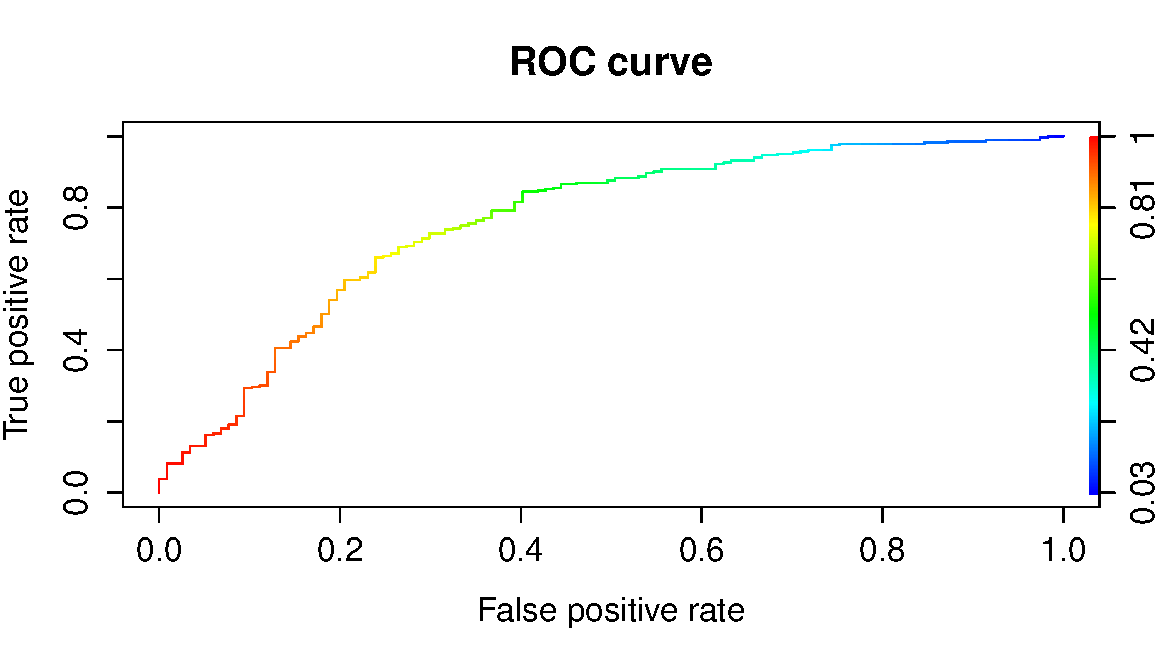
\includegraphics[width=0.98\textwidth]{ROCCurve.pdf}


\subsection*{Lift Curve}
\begin{Schunk}
\begin{Sinput}
> p.rocr.lift <- performance(p.rocr, "lift", "rpp")
> plot(p.rocr.lift, main="Lift Curve", colorize=T)
\end{Sinput}
\end{Schunk}
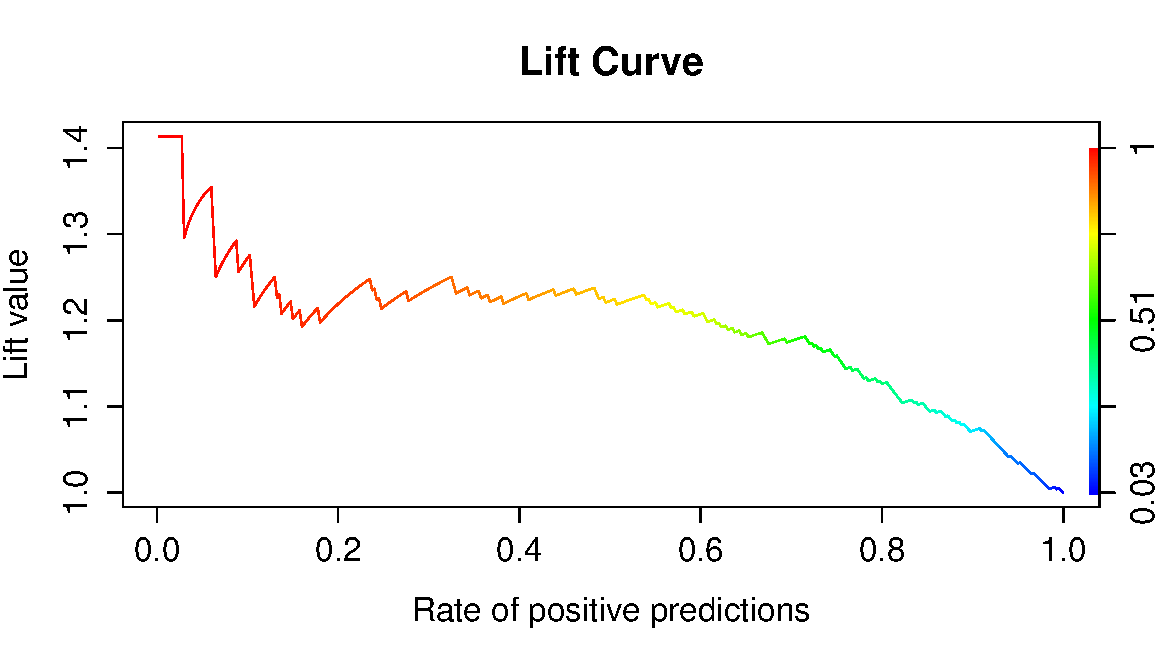
\includegraphics[width=0.98\textwidth]{LiftCurve.pdf}

\subsection{Classification Table with different cutoff values}
\begin{Schunk}
\begin{Sinput}
> calcNetProfit <- function(facts, preds, cutoff) {
+   vals <- sapply(preds, function(y) { ifelse(y<cutoff,0, 1) })  
+   ct <- CrossTable(facts, vals, dnn = c("Actual", "Predicted"))
+   print("Profit with cutoff")
+   print(cutoff)
+   profitFromCrossTable(ct)
+ }
> profitFromCrossTable <- function(ct) {
+   profit <- ct$t[1,1] * 100
+   loss <- ct$t[2,1] * -500
+   profit - loss
+ }
> s <- seq(0,1, by = .1)
> for(i in s) { print(calcNetProfit(gc.test$RESPONSE, p.test, i)) }
\end{Sinput}
\begin{Soutput}
   Cell Contents
|-------------------------|
|                       N |
|         N / Table Total |
|-------------------------|

 
Total Observations in Table:  400 

 
             | vals 
       facts |         1 | Row Total | 
-------------|-----------|-----------|
           0 |       125 |       125 | 
             |     0.312 |           | 
-------------|-----------|-----------|
           1 |       275 |       275 | 
             |     0.688 |           | 
-------------|-----------|-----------|
Column Total |       400 |       400 | 
-------------|-----------|-----------|

 
[1] "Profit with cutoff"
[1] 0
[1] 150000

 
   Cell Contents
|-------------------------|
|                       N |
| Chi-square contribution |
|           N / Row Total |
|           N / Col Total |
|         N / Table Total |
|-------------------------|

 
Total Observations in Table:  400 

 
             | Predicted 
      Actual |         0 |         1 | Row Total | 
-------------|-----------|-----------|-----------|
           0 |         5 |       120 |       125 | 
             |     3.616 |     0.064 |           | 
             |     0.040 |     0.960 |     0.312 | 
             |     0.714 |     0.305 |           | 
             |     0.013 |     0.300 |           | 
-------------|-----------|-----------|-----------|
           1 |         2 |       273 |       275 | 
             |     1.644 |     0.029 |           | 
             |     0.007 |     0.993 |     0.688 | 
             |     0.286 |     0.695 |           | 
             |     0.005 |     0.682 |           | 
-------------|-----------|-----------|-----------|
Column Total |         7 |       393 |       400 | 
             |     0.018 |     0.983 |           | 
-------------|-----------|-----------|-----------|

 
[1] "Profit with cutoff"
[1] 0.1
[1] 1500

 
   Cell Contents
|-------------------------|
|                       N |
| Chi-square contribution |
|           N / Row Total |
|           N / Col Total |
|         N / Table Total |
|-------------------------|

 
Total Observations in Table:  400 

 
             | Predicted 
      Actual |         0 |         1 | Row Total | 
-------------|-----------|-----------|-----------|
           0 |        16 |       109 |       125 | 
             |    12.111 |     0.705 |           | 
             |     0.128 |     0.872 |     0.312 | 
             |     0.727 |     0.288 |           | 
             |     0.040 |     0.273 |           | 
-------------|-----------|-----------|-----------|
           1 |         6 |       269 |       275 | 
             |     5.505 |     0.320 |           | 
             |     0.022 |     0.978 |     0.688 | 
             |     0.273 |     0.712 |           | 
             |     0.015 |     0.672 |           | 
-------------|-----------|-----------|-----------|
Column Total |        22 |       378 |       400 | 
             |     0.055 |     0.945 |           | 
-------------|-----------|-----------|-----------|

 
[1] "Profit with cutoff"
[1] 0.2
[1] 4600

 
   Cell Contents
|-------------------------|
|                       N |
| Chi-square contribution |
|           N / Row Total |
|           N / Col Total |
|         N / Table Total |
|-------------------------|

 
Total Observations in Table:  400 

 
             | Predicted 
      Actual |         0 |         1 | Row Total | 
-------------|-----------|-----------|-----------|
           0 |        32 |        93 |       125 | 
             |    25.642 |     3.089 |           | 
             |     0.256 |     0.744 |     0.312 | 
             |     0.744 |     0.261 |           | 
             |     0.080 |     0.233 |           | 
-------------|-----------|-----------|-----------|
           1 |        11 |       264 |       275 | 
             |    11.656 |     1.404 |           | 
             |     0.040 |     0.960 |     0.688 | 
             |     0.256 |     0.739 |           | 
             |     0.028 |     0.660 |           | 
-------------|-----------|-----------|-----------|
Column Total |        43 |       357 |       400 | 
             |     0.107 |     0.892 |           | 
-------------|-----------|-----------|-----------|

 
[1] "Profit with cutoff"
[1] 0.3
[1] 8700

 
   Cell Contents
|-------------------------|
|                       N |
| Chi-square contribution |
|           N / Row Total |
|           N / Col Total |
|         N / Table Total |
|-------------------------|

 
Total Observations in Table:  400 

 
             | Predicted 
      Actual |         0 |         1 | Row Total | 
-------------|-----------|-----------|-----------|
           0 |        46 |        79 |       125 | 
             |    32.485 |     6.303 |           | 
             |     0.368 |     0.632 |     0.312 | 
             |     0.708 |     0.236 |           | 
             |     0.115 |     0.198 |           | 
-------------|-----------|-----------|-----------|
           1 |        19 |       256 |       275 | 
             |    14.766 |     2.865 |           | 
             |     0.069 |     0.931 |     0.688 | 
             |     0.292 |     0.764 |           | 
             |     0.048 |     0.640 |           | 
-------------|-----------|-----------|-----------|
Column Total |        65 |       335 |       400 | 
             |     0.163 |     0.838 |           | 
-------------|-----------|-----------|-----------|

 
[1] "Profit with cutoff"
[1] 0.4
[1] 14100

 
   Cell Contents
|-------------------------|
|                       N |
| Chi-square contribution |
|           N / Row Total |
|           N / Col Total |
|         N / Table Total |
|-------------------------|

 
Total Observations in Table:  400 

 
             | Predicted 
      Actual |         0 |         1 | Row Total | 
-------------|-----------|-----------|-----------|
           0 |        52 |        73 |       125 | 
             |    28.137 |     7.145 |           | 
             |     0.416 |     0.584 |     0.312 | 
             |     0.642 |     0.229 |           | 
             |     0.130 |     0.182 |           | 
-------------|-----------|-----------|-----------|
           1 |        29 |       246 |       275 | 
             |    12.790 |     3.248 |           | 
             |     0.105 |     0.895 |     0.688 | 
             |     0.358 |     0.771 |           | 
             |     0.072 |     0.615 |           | 
-------------|-----------|-----------|-----------|
Column Total |        81 |       319 |       400 | 
             |     0.203 |     0.797 |           | 
-------------|-----------|-----------|-----------|

 
[1] "Profit with cutoff"
[1] 0.5
[1] 19700

 
   Cell Contents
|-------------------------|
|                       N |
| Chi-square contribution |
|           N / Row Total |
|           N / Col Total |
|         N / Table Total |
|-------------------------|

 
Total Observations in Table:  400 

 
             | Predicted 
      Actual |         0 |         1 | Row Total | 
-------------|-----------|-----------|-----------|
           0 |        73 |        52 |       125 | 
             |    35.390 |    14.809 |           | 
             |     0.584 |     0.416 |     0.312 | 
             |     0.619 |     0.184 |           | 
             |     0.182 |     0.130 |           | 
-------------|-----------|-----------|-----------|
           1 |        45 |       230 |       275 | 
             |    16.086 |     6.731 |           | 
             |     0.164 |     0.836 |     0.688 | 
             |     0.381 |     0.816 |           | 
             |     0.113 |     0.575 |           | 
-------------|-----------|-----------|-----------|
Column Total |       118 |       282 |       400 | 
             |     0.295 |     0.705 |           | 
-------------|-----------|-----------|-----------|

 
[1] "Profit with cutoff"
[1] 0.6
[1] 29800

 
   Cell Contents
|-------------------------|
|                       N |
| Chi-square contribution |
|           N / Row Total |
|           N / Col Total |
|         N / Table Total |
|-------------------------|

 
Total Observations in Table:  400 

 
             | Predicted 
      Actual |         0 |         1 | Row Total | 
-------------|-----------|-----------|-----------|
           0 |        86 |        39 |       125 | 
             |    26.538 |    17.508 |           | 
             |     0.688 |     0.312 |     0.312 | 
             |     0.541 |     0.162 |           | 
             |     0.215 |     0.098 |           | 
-------------|-----------|-----------|-----------|
           1 |        73 |       202 |       275 | 
             |    12.063 |     7.958 |           | 
             |     0.265 |     0.735 |     0.688 | 
             |     0.459 |     0.838 |           | 
             |     0.182 |     0.505 |           | 
-------------|-----------|-----------|-----------|
Column Total |       159 |       241 |       400 | 
             |     0.398 |     0.603 |           | 
-------------|-----------|-----------|-----------|

 
[1] "Profit with cutoff"
[1] 0.7
[1] 45100

 
   Cell Contents
|-------------------------|
|                       N |
| Chi-square contribution |
|           N / Row Total |
|           N / Col Total |
|         N / Table Total |
|-------------------------|

 
Total Observations in Table:  400 

 
             | Predicted 
      Actual |         0 |         1 | Row Total | 
-------------|-----------|-----------|-----------|
           0 |       100 |        25 |       125 | 
             |    22.992 |    22.763 |           | 
             |     0.800 |     0.200 |     0.312 | 
             |     0.503 |     0.124 |           | 
             |     0.250 |     0.062 |           | 
-------------|-----------|-----------|-----------|
           1 |        99 |       176 |       275 | 
             |    10.451 |    10.347 |           | 
             |     0.360 |     0.640 |     0.688 | 
             |     0.497 |     0.876 |           | 
             |     0.247 |     0.440 |           | 
-------------|-----------|-----------|-----------|
Column Total |       199 |       201 |       400 | 
             |     0.497 |     0.502 |           | 
-------------|-----------|-----------|-----------|

 
[1] "Profit with cutoff"
[1] 0.8
[1] 59500

 
   Cell Contents
|-------------------------|
|                       N |
| Chi-square contribution |
|           N / Row Total |
|           N / Col Total |
|         N / Table Total |
|-------------------------|

 
Total Observations in Table:  400 

 
             | Predicted 
      Actual |         0 |         1 | Row Total | 
-------------|-----------|-----------|-----------|
           0 |       113 |        12 |       125 | 
             |     8.986 |    19.316 |           | 
             |     0.904 |     0.096 |     0.312 | 
             |     0.414 |     0.094 |           | 
             |     0.282 |     0.030 |           | 
-------------|-----------|-----------|-----------|
           1 |       160 |       115 |       275 | 
             |     4.084 |     8.780 |           | 
             |     0.582 |     0.418 |     0.688 | 
             |     0.586 |     0.906 |           | 
             |     0.400 |     0.287 |           | 
-------------|-----------|-----------|-----------|
Column Total |       273 |       127 |       400 | 
             |     0.682 |     0.318 |           | 
-------------|-----------|-----------|-----------|

 
[1] "Profit with cutoff"
[1] 0.9
[1] 91300

 
   Cell Contents
|-------------------------|
|                       N |
|         N / Table Total |
|-------------------------|

 
Total Observations in Table:  400 

 
             | vals 
       facts |         0 | Row Total | 
-------------|-----------|-----------|
           0 |       125 |       125 | 
             |     0.312 |           | 
-------------|-----------|-----------|
           1 |       275 |       275 | 
             |     0.688 |           | 
-------------|-----------|-----------|
Column Total |       400 |       400 | 
-------------|-----------|-----------|

 
[1] "Profit with cutoff"
[1] 1
[1] 150000
\end{Soutput}
\end{Schunk}


\section*{Lesson 3 Question and Answer}
\subsection*1\emph{Comments on the models}

\noindent

\subsection*2\emph{If you want to select 275 customers from the validation data set, which model would you adopt for credit rating? Why?}
\newline
\newline
\noindent
With a value for k too small we will classify in a way that is very sensitive to the local characteristcs of the training data.
\newline
\newline
\noindent
With a value of k too large we essentially overfit, ignoring the information contained in the predictor variables. In the extreme with k equal the number of observations in the train data all test data is assigned to the most frequent class in the train data, Owner in the present case. 

\end{document}
